% !TEX encoding = UTF-8 Unicode
%!TEX root = thesis.tex
% !TEX spellcheck = en-US
%%=========================================
\chapter{Method}
\label{ch:chapter2}


To fulfill the goal of this thesis, an experiment to compare the energy use of different JavaScript engines was developed. Using a independent power supply, giving a stable voltage, and then measure the current drawn from the hardware platforms while executing programs run in a JavaScript engine.
These measurements can be used to find the power used by a single program, and by running the program a large number of times, an average power consumption of the program can be obtained.
All of the programs are trivial operations in a loop, and using the average consumption, the energy cost of a single expression in the JavaScript engine can be found.

The goal of the experiment is to look at differences in the energy use of the different JavaScript implementations, which means that it is not the exact numbers that are of interest, but rather the trends that the numbers show.
For the experiment, this translates to being approximate whenever it is appropriate.


\subsection{Programs}
Four programs were used on each tested platform, all following a similar pattern: In a loop repeated 1,000,000 times, some expression is evaluated.
The programs are named  are addition, multiplication, closure and bit shift; testing various JavaScript features.
The addition program can be seen in \fref{lst:add}


\begin{lstlisting}[language=JavaScript,caption={Addition program}, label={lst:add}]
for(var i = 0; i < 1000000; i++) {
        var a = 1;
        var b = 2;
        var c = a + b;
}
\end{lstlisting}



%http://git-public.pengutronix.de/?p=OSELAS.BSP-EnergyMicro-Gecko.git;a=summary

\section{Hardware Platforms}

\begin{table}[h]
\centering
\begin{tabular}{| c | c | c |}
\hline
            & Raspberry Pi  & Tessel        \\ \hline
CPU         & BCM2835       & LPC1830       \\ \hline
Core        & ARM1173       & ARM Cortex M3 \\ \hline
Architecture& ARMv6         & ARMv7         \\ \hline
Clock Speed & 700 MHz       & 180 MHz       \\ \hline
RAM         & 512 MB        & 32 MB         \\ \hline
Flash       & SD-card       & 32 MB         \\
\hline
\end{tabular}
\caption{Comparing a Tessel 1 with a Raspberry Pi 1 Model B}
\label{tab:specs}
\end{table}


As can be gathered from \fref{tab:specs}, the Raspberry Pi is a much faster machine than the Tessel, clocked almost 4 times higher, and with 16 times the amount of RAM.
This means that the Raspberry Pi is able to run much bigger software and do it faster, but also that it will use a lot more power.

\subsection{Silicon Labs EFM32GG STK3700}

\section{Software Platforms}
\subsection{Tessel}
The goal of the Tessel\footnote{https://tessel.io} platform is to be an easy way of giving new developers access to hardware programming.

One of the rationales behind choosing Lua as the intermediate language (and the Tessel 1 way of running code on a microcontroller) was that Lua has a low memory profile and is generally embeddable.
At the time, the only choice in JavaScript engine was the V8 engine, and the goal for Tessel was to cater for low energy use.
The next step in this direction was to use LuaJIT to get a much more optimized running of programs.(\cite{newengine})

To be able to write JavaScript and run it as Lua, the JavaScript code needs to be translated.
In the Tessel stack, the Colony Compiler\footnote{https://github.com/tessel/colony-compiler} does this translation, using simple lexical parsing, i.e. changing JavaScript features directly into Lua equivalents.

Running now on the Tessel is the LuaJIT virtual machine, which is much faster than the standard Lua engine, due to a more efficient design. While there was a goal to enable the just-in-time compilation, the developers of Tessel has since decided that some of the goals of the project can’t be reconciled with a real low power usage, and the next version of Tessel will run node/io.js.(\cite{movingfaster})

\subsection{Espruino}
Espruino\footnote{http://www.espruino.com/} has, in addition to the goal of Tessel to bring hardware to new people, also the goal of doing it as efficient as possible.
The implementation is targeted to devices with memory as small as 128kB Flash and 8kB RAM, way less than both hardware platforms that are used in this experiment provides.
To achieve this goal, a number of tradeofs has been done to the implementation.

The Espruino VM is an almost complete JavaScript implementation, missing some elements due to the memory limits imposed by the design goal. 
Mainly, the big difference between Espruino and other JavaScript implementations, is that it does not translate the source code to byte code, but executes the source directly. 
This is again due to memory concerns, as the developers want the source code to be on the device when executing, to be able to edit the source code on the device. 
If the VM translated to byte code, it would need twice the storage for the same program to keep it all on the device.

Other optimizations done for memory minimization (and thus speed) include using a linked list for storage of arrays and objects (allowing for constant time insertion and deletion) and including typed arrays, which is a direct mapping of memory to the data structure.

While the platform itself is designed to be power efficient, it does not optimize the code before running it, requiring the programmer to write efficient code. 
Adding some middleware to optimize code before running it on the Espruino could help minimizing the energy use.


\subsection{io.js/node.js}
Node.js/io.js\footnote{https://iojs.org} is developed to run JavaScript on computers, using the V8 Engine, found in browsers such as Google Chrome.
As the normal running environments for Node are not restricted on energy, the platform is optimized for speed.
This does not mean that the platform is power hungry, as speed optimizations might lead to better energy efficiency as well.
In fact, Technical Machine has announced that they will use io.js for the Tessel 2, that will release in the fall of 2015.(\cite{movingfaster})

In this experiment, the Node.js fork io.js will be used, as it is currently more updated than Node.js.
The io.js team has recently announced that they will be joining the new Node Foundation, and the project that is currently io.js, will be renamed Node in the near future.
While this brings a bit of terminology problems in this thesis, when either io.js or Node.js is mentioned, it can be assumed that it is io.js that is used.


\subsection{Linux}
To run programs on the Raspberry Pi, an operating system is needed, 
The Raspbian OS, based on the Debian Linux distribution, 

Provided with the Raspberry Pi is the Raspbian OS, based on the Debian Linux distribution.


% http://sjoerd.luon.net/posts/2015/02/debian-jessie-on-rpi2/



\section{Experimental setup}

\begin{figure}[ht]
\centering
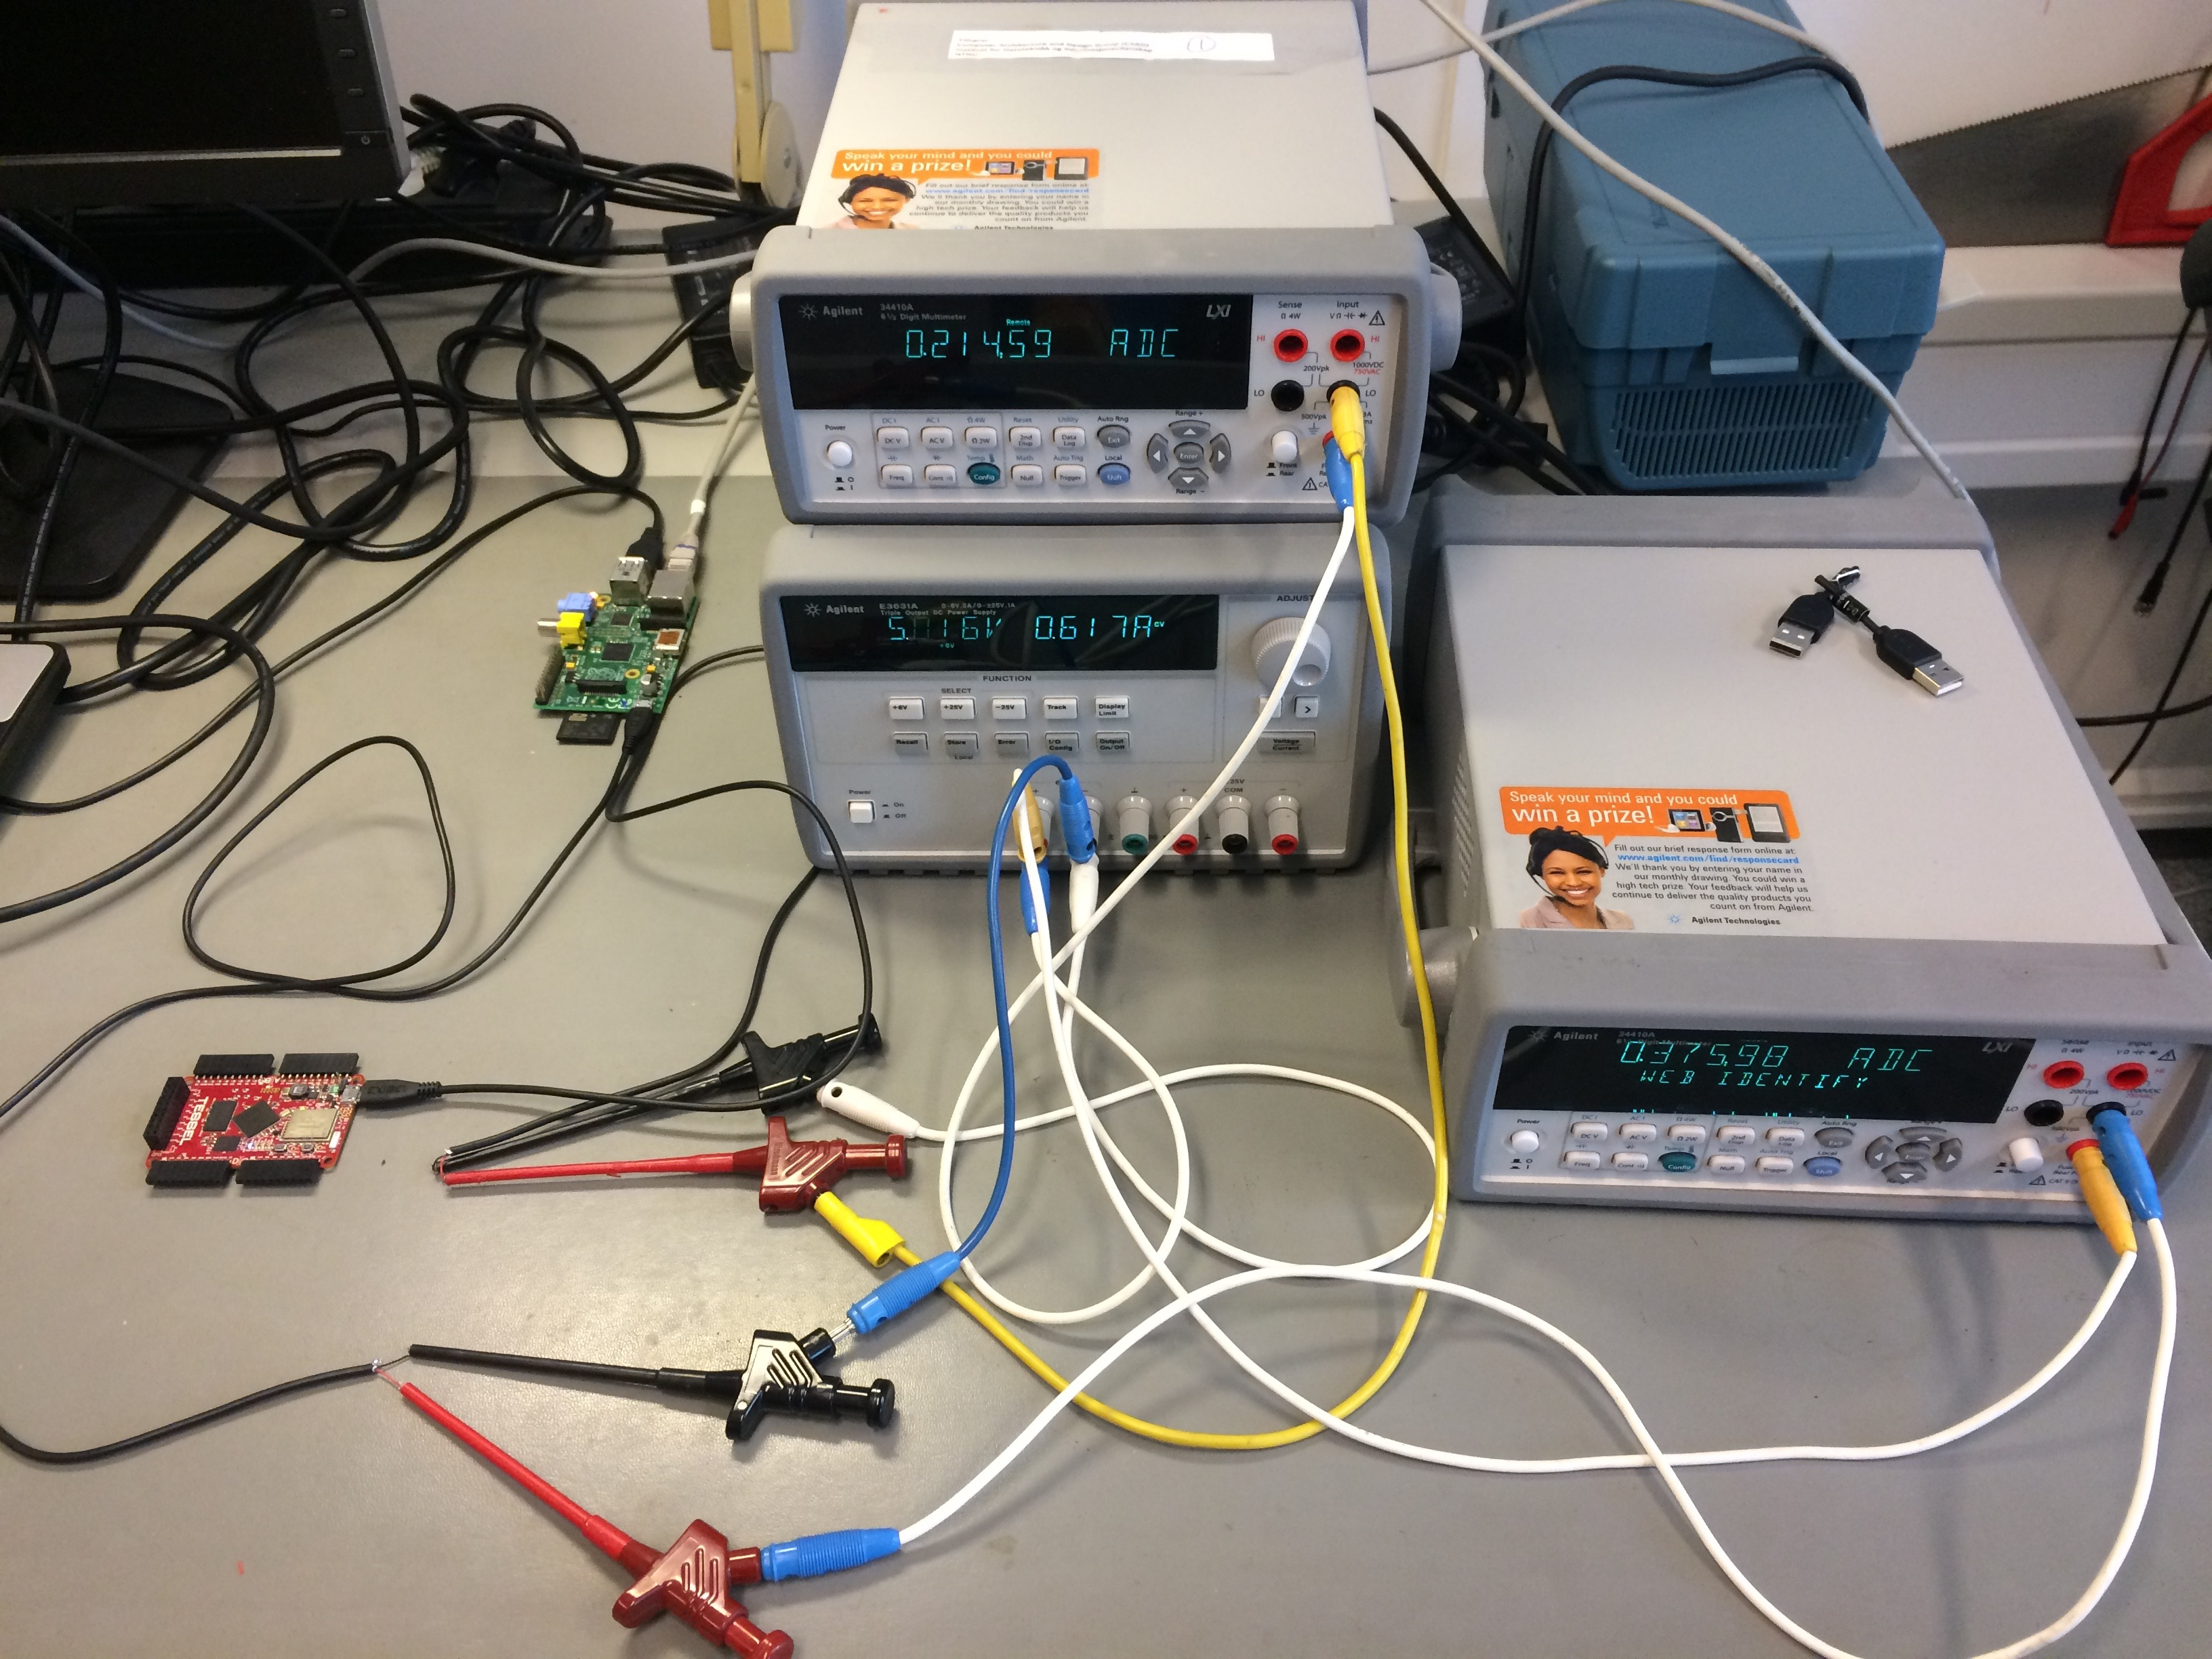
\includegraphics[width=\textwidth]{fig/pics/setup.jpg}
\caption{The hardware setup of the experiment}
\label{fig:setup}
\end{figure}

To power the experiment, the Agilent E3631A was used. 
As both the hardware platforms were running experiments at the same time, they were both connected to the power supply, with a common ground. 
The multimeter, Agilent 34410A, was connected in series between the power supply and the device, set to ADC measurement. 
There was one multimeter for each device while running in parallel.
Both devices receives power through a Micro USB cable.
A cable was cut up, and using clamps, the power and ground wires were connected to the power supply.(\cite{usbmicro})

The multimeter supports logging over LAN, allowing to remotely monitor the experiment.
Using the Keysight Benchvue Software, all measurements can be exported in CSV format.
Together with the Raspberry Pi's remote SSH-access, the experiments on the Pi can be remotely started and controlled.
To fully automate the experiment on the Raspberry Pi, a shell script was written to restart the program for as many times that was required in the experiment.
After each run, the device would sleep for 0.5 seconds before the reset, to differ between each run while running.

Unlike the Raspberry Pi, the Tessel hardware does not allow for remote access while it is running on external power, because the USB port is the only communication port able to flash the Tessel.
To work around this problem, the program was written to the internal flash, which will start to run whenever the Tessel boots.
Then the hardware was reset from software after each program run.
This feature did not exist in the platform, but was written for this experiment, and has since been accepted into the project.\footnote{\url{https://github.com/tessel/t1-firmware/pull/140}}
After approximately the wanted number of runs were done, the logging was stopped.

Another way of doing it could have been to create an USB cable with only data wires from a computer and connect those to the data wires on the cable going to the device. \textcolor{red}{Should I mention this?}


\subsection{Data manipulation}
The Benchvue Software can export the measurement data in CSV format, in two columns with time stamp and the sampled data at that time stamp.
These files were read in a Python program, which did the manipulations needed on the data.

To find the average power consumption of every run on Raspberry Pi, the fact that the current drawn while it was sleeping was always under 0.39 m/micro A, and always above when the program was running, was exploited. 
Stripping away everything under this threshold, and splitting this stream up into blocks of as many samples as the average program contains, the energy consumed by each program in the run can be added up to. 
The average of these sums is then the average power usage of one experiment.

The Tessel data was not as easy to manipulate, as the board reset procedure is not as clear when it begins and ends from the current data. To get a similar data set to work on as from the Raspberry Pi, as many samples as go into the board reset is removed after the number of samples of the average program is    removed.

